%%%%%%%%%%%%%%%%%%%%
%% KAPITEL Server %%
%%%%%%%%%%%%%%%%%%%%
%% JONAS (Hilfe: Steffen)
%%%%%%%%%%%%%%%%%%%%%
\section{Server}

\subsection{Applikationsserver}
\label{sec:app-server}

\subsection{Storageserver}
\label{sec:stor-server}

\subsection{Betriebssysteme}
\label{sec:server-os}

\section{SAP NetWeaver Plattform}
\label{sec:netweaver}

%%%%%%%%%%%%%%%%%%%%%%%
%% KAPITEL Datenbank %%
%%%%%%%%%%%%%%%%%%%%%%%
%% STEFFEN
%%%%%%%%%%%%%%%%%%%%%%%
\section{Datenbank}

\subsection{SAP HANA}
\label{sec:db-hana}

\subsubsection{Einführung}
\label{sec:db-hana-intro}
% historische, hana studio, rowstore (anderer Aufbau als bei herkömml. dbs)
\gls{sap} \gls{hana} kombiniert die Funktionen einer \gls{db}, der Datenverarbeitung und die Funktionen einer Anwendungsplattform auf Ebene des Hardware Arbeitsspeichers. \gls{hana} bietet \gls{ua} Bibliotheken für Vorhersage, Planung, Textanalyse oder Geschäftsanalysen an.\\

\begin{figure}[H]
	\begin{center}
	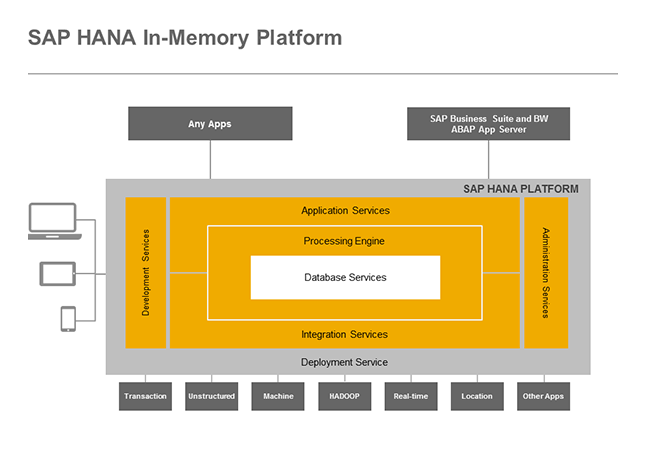
\includegraphics[width=1\linewidth]{grafiken/hana-features-overview.png}
	\vspace{-20pt}
	\caption{Aufbau der \gls{sap} \gls{hana} Plattform \cite{SAPHanaAbout}}
	\vspace{-10pt}
	\label{abb:SAPHanaAbout}
	\end{center}
\end{figure}

\gls{hana} verwendet in seiner \gls{db} einen sogenannten spaltenbasierten Datenspeicher, welcher im Arbeitsspeicher abgespeichert wird. Dieser Datenspeicher ist durch verschiedene Sicherheitsfeatures vor Datenverlust bei Stromausfall oder ähnlichem gesichert.
Dadurch, dass Anwendungen direkt auf der \gls{hana} Instanz ausgeführt werden können, vereinfacht es die Entwicklung von Applikationen im Umfeld von großen Datenquellen und Datenstrukturen. In Abbildung \ref{abb:SAPHanaAbout} ist die Struktur von \gls{hana} abgebildet.

\subsubsection{Hands On}
\label{sec:db-hana-ho}
% welche wichtigen Befehle gibt es

\subsubsection{Vergleich}
\label{sec:db-hana-vgl}
% zeitvergleich oracle / hana db select

\subsection{Sonstige}
\label{sec:db-sonstige}
% welche datenbanken kann man sonst benutzen
% oracle,...